\documentclass{beamer}

\mode<presentation> {
        \usetheme{Dresden}
        \usecolortheme{seahorse}
        \setbeamercovered{transparent}
}
\usepackage[utf8]{inputenc}
\usepackage[czech]{babel}
\usepackage{graphicx}
\usepackage{hyperref}
\usepackage{lipsum}
\usepackage{amsmath,amsfonts,amssymb}
\graphicspath{{images/}}
\usepackage[skip=1pt,figurename=,justification=centering]{caption}

\title{LSTM SÍTĚ}
\subtitle{SOČ obor č. 18: informatika}
\institute{Gymnázium Brno-Řečkovice Terezy Novákové 2, p. o.}
\author{Jakub Šťastný}
\begin{document}
        \setbeamertemplate{headline}{}

	%Title


        \begin{frame}
            \titlepage
        \end{frame}
        \begin{frame}
                \frametitle{Osnova}
                \tableofcontents
        \end{frame}



	%Cíle



	\section{Cíle práce}
	\begin{frame}
        \frametitle{Cíle práce}
        	\begin{itemize}
			\item Nastudovat, pochopit a shrnout základy neuronových sítí a sítí LSTM
			\item Vytvořit a naučit funkční LSTM síť
			\item Naučit síť generovat text a demonstrovat tak, jak funguje učení LSTM sítí
        	\end{itemize}
	\end{frame}

	%Neuronové sítě


	\section{Neuronové sítě}
	\begin{frame}
	\frametitle{Neuronové sítě}
		\begin{itemize}
			\item Jedna z technik strojového učení a umělé inteligence
			\item Inspirace v biologických strukturách
			\item Základní jednotka je neuron, který se spojuje do sítí
			\item Mají schopnost se samy učit
			\item Používají se v situacích, kdy není potřeba nebo naopak nelze znát 100\% přesný výsledek
		\end{itemize}
		\begin{figure}
			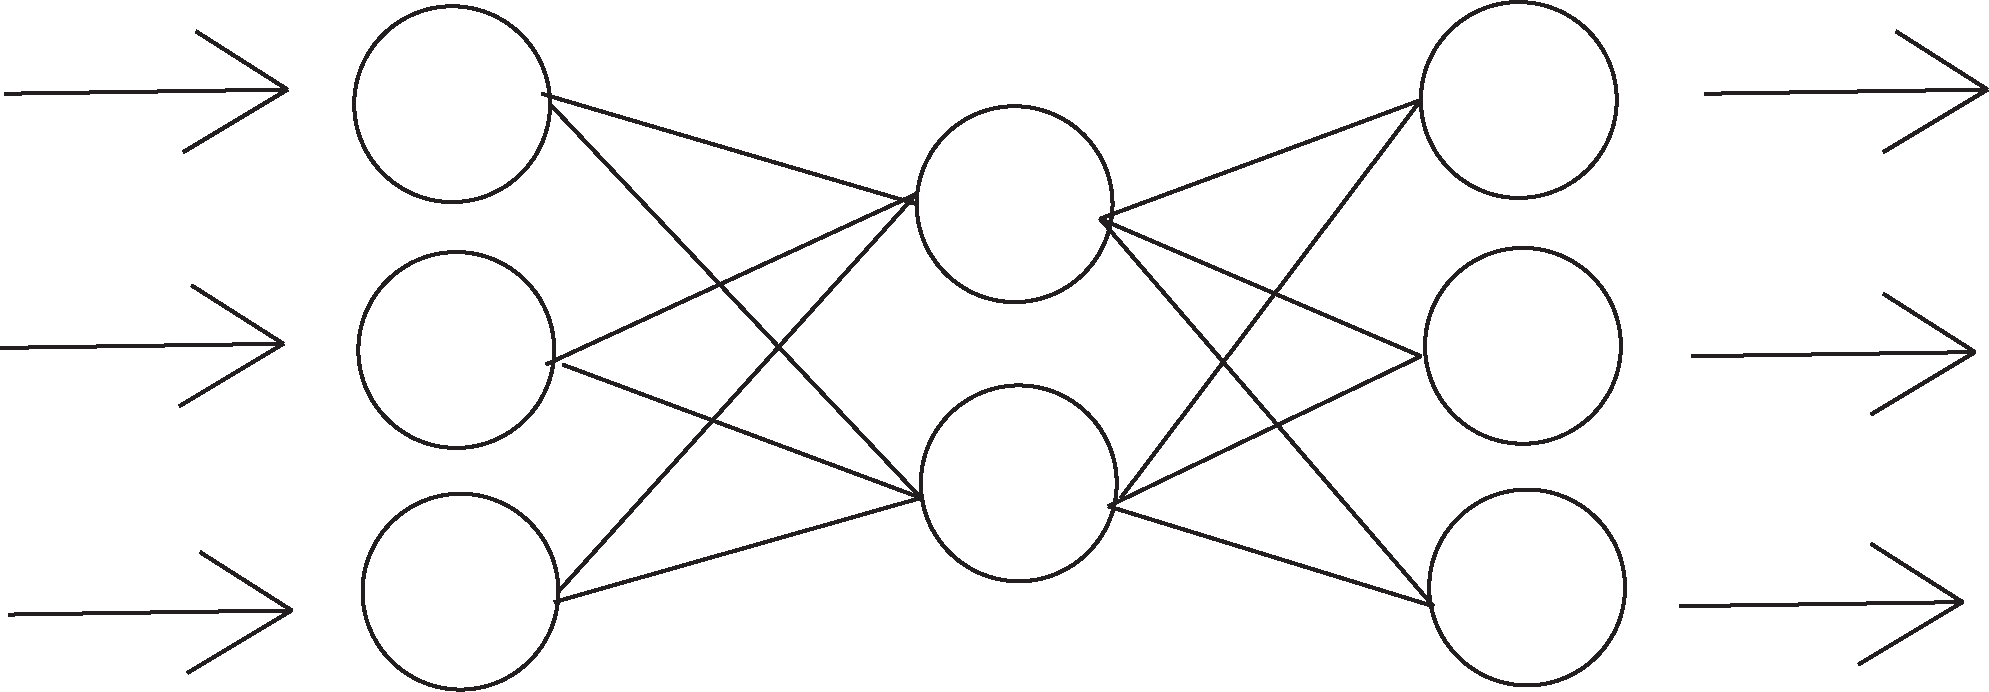
\includegraphics[height=3cm]{neuralNetwork.png} 
			\caption{{\fontsize{5}{6}\selectfont zdroj vlastní}}
		\end{figure}
	\end{frame}
	

	%LSTM síť


	\section{LSTM síť}
	\begin{frame}
	\frametitle{LSTM síť}
		\begin{columns}[t]
			\column{5cm}
			\begin{itemize}
				\item Vstup je uspořádaná množina reálných čísel
				\item Výstup je reálné číslo
				\item Vstup ohodnocen vahami 
				\item Obsahuje vnitřní stav
				\item Obsahuje 3 brány\\(input, output a forget)
			\end{itemize}
			\column{7cm}
			\begin{figure}
				\centering
				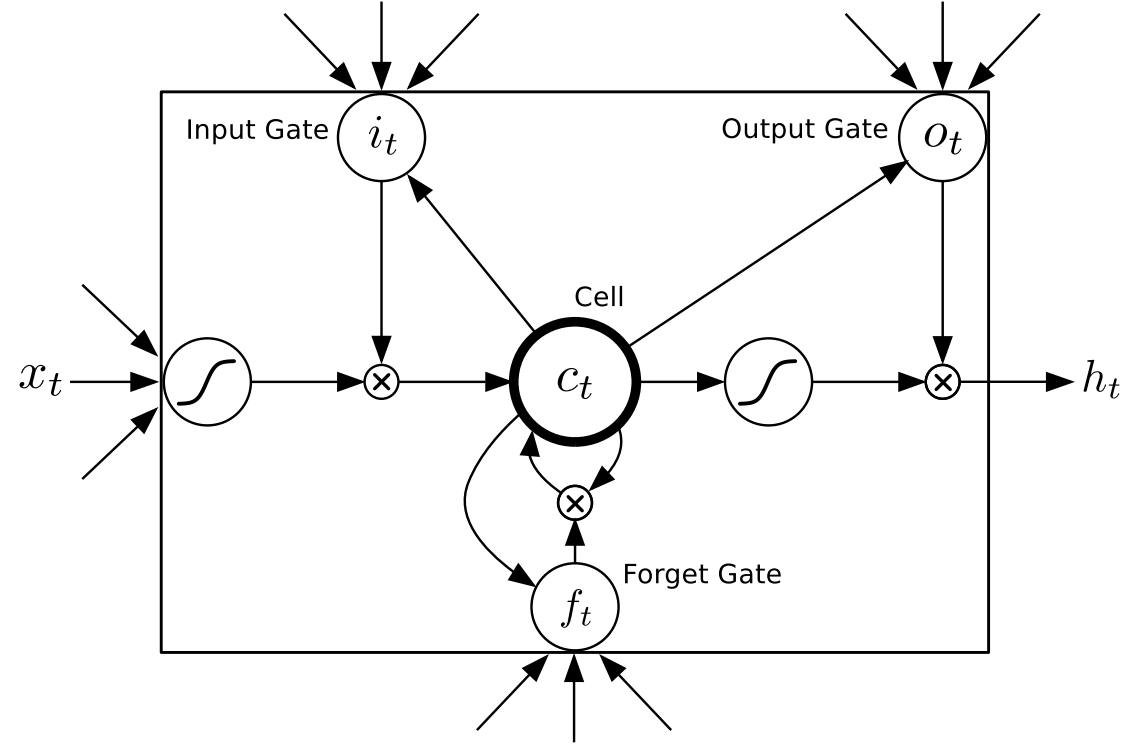
\includegraphics[width=7cm, height=4.3cm]{LSTM-cell.png}\\ %http://blog.otoro.net/wp-content/uploads/sites/2/2015/05/LSTM.png
				\caption{{\fontsize{5}{6}\selectfont\url{http://blog.otoro.net/wp-content/uploads/sites/2/2015/05/LSTM.png}}}
			\end{figure}
		\end{columns}
		\begin{columns}
			\column{5cm}
				$o = g_o(s_0 + g_i \cdot \tanh(\sum\limits_{i=0}^nw_ix_i))$
			\column{5cm}
				$s = g_f(s_0 + g_i \cdot \tanh(\sum\limits_{i=0}^nw_ix_i))$
		\end{columns}
	\end{frame}
	
	
	%Učení sítí


	\section{Učení sítě}
	\begin{frame}
	\frametitle{Učení sítě}
		\begin{itemize}
			\item Back propagation through time (s učitelem)
			\item Určíme chybovou funkci $J: \mathbb{R}^n \rightarrow \mathbb{R}$, kterou minimalizujeme
		\end{itemize}
		\begin{figure}
			\centering
			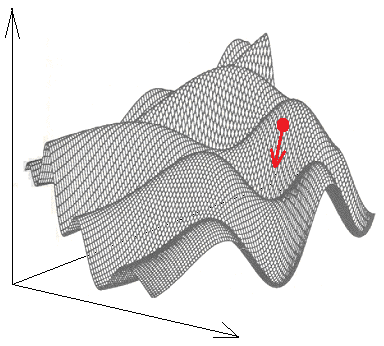
\includegraphics[width=7cm, height=5cm]{backpropagation.png} %http://i.iinfo.cz/images/49/biologicky-inspirovane-5-1.png
			\caption{\fontsize{5}{6}\selectfont\url{http://i.iinfo.cz/images/49/biologicky-inspirovane-5-1.png}}	
		\end{figure}
	\end{frame}


	%Vlastní síť


	\section{Vlastní síť}
	\begin{frame}
	\frametitle{Vlastní síť}
		\begin{itemize}
			\item C\#
			\item .Net Framework 3.6 nebo vyšší
			\item Sharp-ML-Recurrent
			\item klasifikační síť
			\item 2 skryté vrstvy o 128 neuronech typu LSTM
			\item výstupní vrstva typu FeedForward s aktivační funkcí sigmoid
		\end{itemize}
		\begin{figure}
			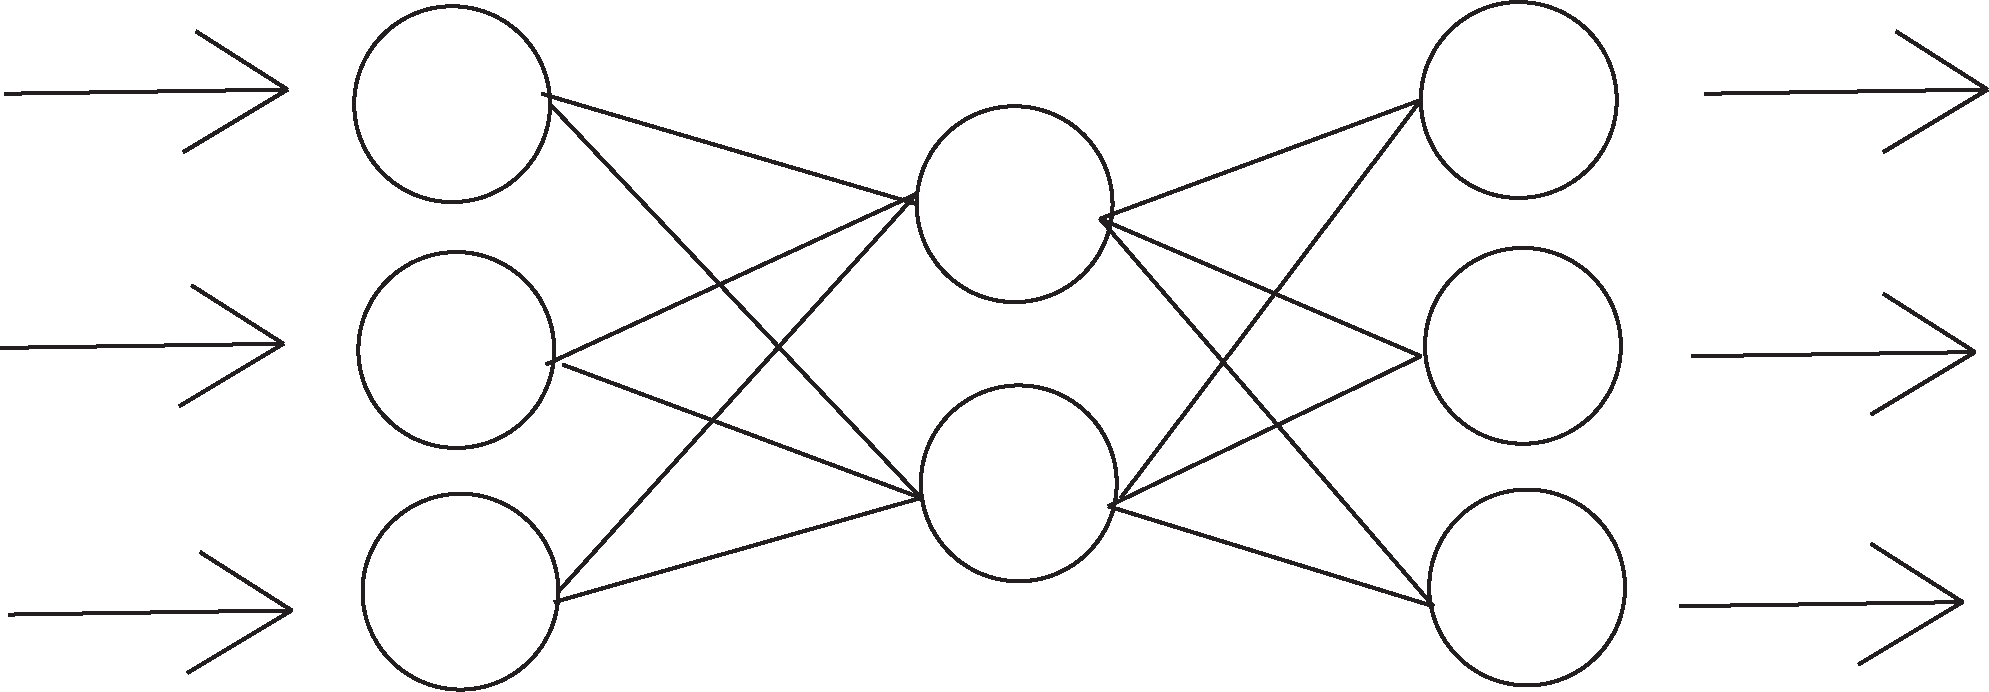
\includegraphics[height=3cm]{neuralNetwork.png}
			\caption{{\fontsize{5}{6}\selectfont zdroj vlastní}}
		\end{figure}
	\end{frame}
	

	%Výsledky učení


	\section{Výsledky učení sítě}
	\begin{frame}
	\frametitle{Výsledky učení sítě}
		\begin{itemize}
			\item Studijní data - Shakespeare
			\item Počet epoch - 50, Learning rate - 0,0012 (0,85)
		\end{itemize}
		\begin{block}{Výsledky po 1. epoše}
			\begin{quote}
				sed, stasent. bisints ore blowd wencilow.\\
				t you sils. out daceigas\\
				n, stish may\\
				d,\\
				or matter\\
				ivits, heav bowe\\
				wks\\
				s~tencoudes fonds but.\\
			\end{quote}
		\end{block}
	\end{frame}

	\begin{frame}
	\frametitle{Výsledky učení sítě}
		\begin{itemize}
			\item Studijní data - Shakespeare
			\item Počet epoch - 50, Learning rate - 0,0012 (0,85)
		\end{itemize}
		\begin{block}{Výsledky po 4. epoše}
			\begin{quote}
				e damit hither. such sir\\
				on he him:\\
				him my hid tho wools: hand,\\
				e, home: yat marich.\\
				it whils, musice our\\
				dom. feeres out whist wides\\
				om wont storls, lie,\\
				ition it. sit, if it\\
			\end{quote}
		\end{block}
	\end{frame}

	\begin{frame}
	\frametitle{Výsledky učení sítě}
		\begin{itemize}
			\item Studijní data - Shakespeare
			\item Počet epoch - 50, Learning rate - 0,0012 (0,85)
		\end{itemize}
		\begin{block}{Výsledky po 12. epoše}
			\begin{quote}
				you, wash horted seads, alath\\
				s~saftiman on. are wand marian\\
				de and relord had hit. of off hold. stolding, but wont, a\\
				telong, his\\
				wrong.\\
				s~friend, whiles\\
				a touth mind\\
				out flath. \\
			\end{quote}
		\end{block}
	\end{frame}

	\begin{frame}
	\frametitle{Výsledky učení sítě}
		\begin{itemize}
			\item Studijní data - Shakespeare
			\item Počet epoch - 50, Learning rate - 0,0012 (0,85)
		\end{itemize}
		\begin{block}{Výsledky po 23. epoše}
			\begin{quote}
				-henre, brothes\\
				drough, i margan as all or\\
				or; too i may, nate,\\
				end his\\
				n, were at himsel; my\\
				u~arced;\\
			        in yet; can i wash bust thine.\\
				our, than that holland:\\
			\end{quote}
		\end{block}
	\end{frame}


	%Závěr


	\section{Závěr}
	\begin{frame}
	\frametitle{Závěr}
		\begin{itemize}
			\item Všechny cíle byly splněny
			\item Shrnul a pochopil jsem fungování sítí LSTM
			\item Vytvořil jsem funkční síť, pro generování textových dat
			%\hspace[1cm]
			\item Kroky do budoucna:
			\begin{itemize}
				\item Přepracovat síť na generování hudby
				\item Vypracovat webovou aplikaci a publikovat na ni svoji práci
			\end{itemize}
		\end{itemize}
	\end{frame}
	
	
	%Poděkování


	\begin{frame}
	\frametitle{Poděkování}
		\begin{center}
			{\LARGE Mgr. Jan Herman}
		\end{center}
	\end{frame}

	\begin{frame}
		\frametitle{Poděkování}
		\begin{center}
			{\LARGE DĚKUJI ZA POZORNOST}
		\end{center}
	\end{frame}

\end{document}
